\subsection{Model overview}
To model the metabolic the interaction of multiple species populations, each individual was represented as an agent on a grid environment (Figure \hyperref[fig:bacarena]{\ref{fig:bacarena}}).
\begin{figure}[h!]\centering
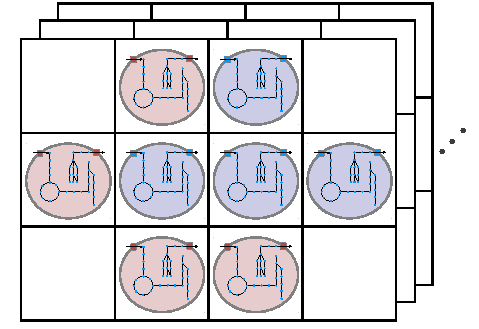
\includegraphics[scale=1.4]{method_chart_BacArena.pdf}
\caption[Overview BacArena]{Overview of the grid environment with two different bacterial agent types (species) in red and blue. Each substrates has its own grid representation.}
\label{fig:bacarena}
\end{figure}
The grid environment was composed of different metabolite concentrations.
Furthermore, the species type was recorded for each agent to call the respective genome-wide metabolic reconstruction in every iteration (Algorithm \hyperref[alg:mainloop]{\ref{alg:mainloop}}). The constraints for the subsequent fba were set according to the current metabolite concentrations of the grid cell, where the respective agent was located.
\begin{algorithm}
\caption{Main model iterations called by \texttt{diffbac.R} with the different functions applied to bacterial agents and metabolite concentrations.}
\SetAlgoLined
\For{number of iterations}{
  \emph{diffusion}()\;
  \For{number of bacteria}{
    \emph{fba}()\;
    \emph{movement}()\;
    \emph{growth}()\;
  }
}
\label{alg:mainloop}
\end{algorithm}
The solution of the fba was used to adjust the biomass of each agent and to modify the metabolite concentrations according to the produced products and consumed substrates. 
This uptake and output of metabolites constitute the exchange with the virtual environment.
A diffusion model was applied to spread the metabolite concentrations over the grid environment and a movement function allowed the random dispersal of each bacterial agent.

A central theme of \texttt{BacArena} was the modularity of each funcsubtion and metabolic model to allow the extension and replacement of certain parts of the framework. Furthermore, the modularity also enables the inclusion of any desired amount of microbial species. In the following sections the modules of \texttt{BacArena} will be regarded more closely. 

\subsection{Representation}
% -> this should be part of the discussion:
%Implementation began in \textit{netlogo}, which is a simple and wide-used agent based modeling framework.\cite{Wilensky1999}
%For statistical analysis the powerful \textit{R} language was our choice. 
%There exists joint package for interaction of \textit{R} and netlogo (e.g.: \cite{Thiele2010}), but above all speed limitations led us looking for other possibilities.
%In \textit{R} there exists packages to do agent based modeling e.g. \textit{simecol}, which is an ecological framework with differential equation based approach, too. \cite{Petzoldt2007}.
%But again we could retain performance improvement by simply implementing it ourselves directly in \textit{R}.
The main parts of the framework were implemented in the programming language \texttt{R} ( *). Additionally, certain parts were implemented in \texttt{C++} and integrated in \texttt{R} with the package \texttt{Rcpp} ( *).

\subsubsection{Environment \& Grid}
Agents in \texttt{BacArena} were assigned to specific two-dimensional $n \times m$ grid positions $i, j \in \mathbb{N}$ and a type variable indicating the species. The grid is a discretization of space and could be imagined as a chess board, where the agents can move like chess pieces. 
One single part of the grid is called \textit{cell} with no biological meaning.
For each grid positions certain metabolite concentrations were also recorded and stored in a separate matrix. For each metabolite a own matrix was constructed (Figure \hyperref[fig:bacarena]{\ref{fig:bacarena}}). The bacterial agents could interact with this environment by the consumption and production of metabolite concentrations.
Attention is necessary for the boundaries of the grid.
Here continuous boundary conditions were choosen, i.e. rectangle grid is forming a surface of a torus/donut (horn-torus in square case).

\subsubsection{Bacteria}
Bacteria were represented as rows in a matrix, which had four columns and rows according to the current number of agents on the grid. The first two columns contained the discrete positions of the agents on the grid. The third column indicated the species type of the respective agent. The fourth column stored the current biomass value of the agents.

For certain bacterial species published genome-wide metabolic reconstruction were used as a representation of the individual metabolism and to perform the flux balance analysis. In the present study the \emph{Escherichia coli} ( *), \emph{Methanosarcina barkeri} ( *) and \emph{Clostridium beijerinckii} ( *) \textit{SBML} model were used. For each model the metabolites of the published artificial minimal medium (except the metabolites mentioned below) were set to concentrations, which were always present.

In each iteration in \texttt{diffbac.R} (Algorithm \hyperref[alg:mainloop]{\ref{alg:mainloop}}), rows were deleted and included according to the growth function (see below). The grid positions were updated according to the movement function and the biomass increase as a solution of the fba was added to the current biomass value for each agent.

\subsubsection{Substrate}
Metabolite concentrations were represented as matrices $m_s \in \mathbb{R}^{n \times m}$ for all substrates $s$. According to the requirements of the used genome-wide metabolic models certain metabolites were selected. In the present study these metabolites were: acetate, aketoglutarate, carbon dioxide, ethanol, formiate, fumarate, glucose, water, proton, lactate, oxygen, phosphate, pyruvate, succinate, hydrogen, methanol, methane, acetone, butyrate and butanol.
This could be extended easily by just adding another substrate matrix.
Nonetheless it's necessary to define the corresponding exchange reaction for all organisms for this new added metabolite because there exists no common nomenclature.

The entries of the metabolite matrices were initialized with a concentration of 70 mmol per grid cell. Additionally, in certain simulations the concentration was of selected metabolites set to 0 mmol to generate diverse metabolic phenotypes, such as anaerobic metabolisms.

\subsection{Interactions as rules}
The different representations were closely integrated with rules, which acted on each individual level.

\subsubsection{Movement}
\begin{algorithm}
\caption{Movement of bacterial agents in the von Neumann neighbourhood with $i$ and $j$ as the current positions on the grid}
\SetAlgoLined
$a \leftarrow i+random(1,-1)$\;
$b \leftarrow j+random(1,-1)$\;
\For{number of bacteria}{
	\uIf{$($a,b$)$ $\in$ bacteria positions}{do not move}
    \Else{$i \leftarrow a$\;
    $j \leftarrow b$\;}
}
\end{algorithm}

\subsubsection{Diffusion}
In agent based modeling there are two different rules for updating.
A Synchronous mode updates all cells simultanously, i.e. local changes are stored in a temporary copy and only after computation of all cells this changes will be efficacious.
Contrary to this, in a asynchronous mode changes will be made immediately (\cite{Matthies2002} p. 92).\\
Implementing a simple, naive diffusion model, which interchanges states between neighboured cells, asynchronous updating with randomly choosen cells is preferred because i) synchronouse updating violates conservation laws and ii) nonrandomly asynchronousy is causing a biased diffusion direction \cite{Bandman1999}.
\begin{algorithm}
  \caption{Diffusion is implemented in c++ using Rcpp}
  \SetAlgoLined
  \For{all substrates s}{
    $l \leftarrow 0$\;
    $n \leftarrow$ rows\;
    $m \leftarrow$ columns\;
    \While{$l++ < n \cdot m$}{
      $i \leftarrow random(1,n)$\;
      $j \leftarrow random(1,m)$\;
      $\min$ $\leftarrow$ random local minimum in neighbourhood of cell $i,j$\;
      $m \leftarrow (s(\min_i, \min_j)+s(i,j))/2$\;
      $s(i,j) \leftarrow m$\;
      $s(\min_i, \min_j) \leftarrow m$\;
    }
  }
\end{algorithm}
Further work could be done by implementing more sofisticated diffusion models like block-rotation \cite{Bandman1999} or the discrete diffusion model by Grajdeanu \cite{Grajdeanu2007}.


\subsubsection{Flux balance analysis}

\subsubsection{Growth}
\paragraph{Duplication}
For each organism it's obligatory to define maintenance.
Allways some non growth associated maintenance (ngam) is needed, which accounts normal energy consumption for upkeeping the cell.
During growth there is additionally some growth associated maintenance (gam) to describe energy consumption necessary to replicate the cell. The unit for ngam and gam is $mmol/g_{\texttt{dryweight}}/h^{-1}$\cite{Thiele2010}.\\
In \texttt{BacArena} all cells start with a biomass of $1$ symbolizing a intact cell.
Flux balance analysis (fba) estimates fluxes and returns especially a maximized flux through the biomass function.
This biomass flux is added to the initial biomass value. A serie of such steps symbolizes groth.
If accumulated biomass reaches twice the initial biomass value, duplication is possible
\paragraph{Death}
Flux balance analysis considers a fixed ngam flux and growth depending gam part of the biomass function.
Under starving conditions, where no fluxes according to fba calculations can be found, we consider the current biomass as reservoir, from which the cell can feed on.
\[
  \textrm{biomass}_{\,t+1} = -\frac{\textrm{ngam}}{\textrm{gam}}\cdot \textrm{biomass}_{\,t}+\textrm{biomass}_{\,t}
\]
